\begin{figure}[!b]
    \centering
    \hspace*{-.7cm}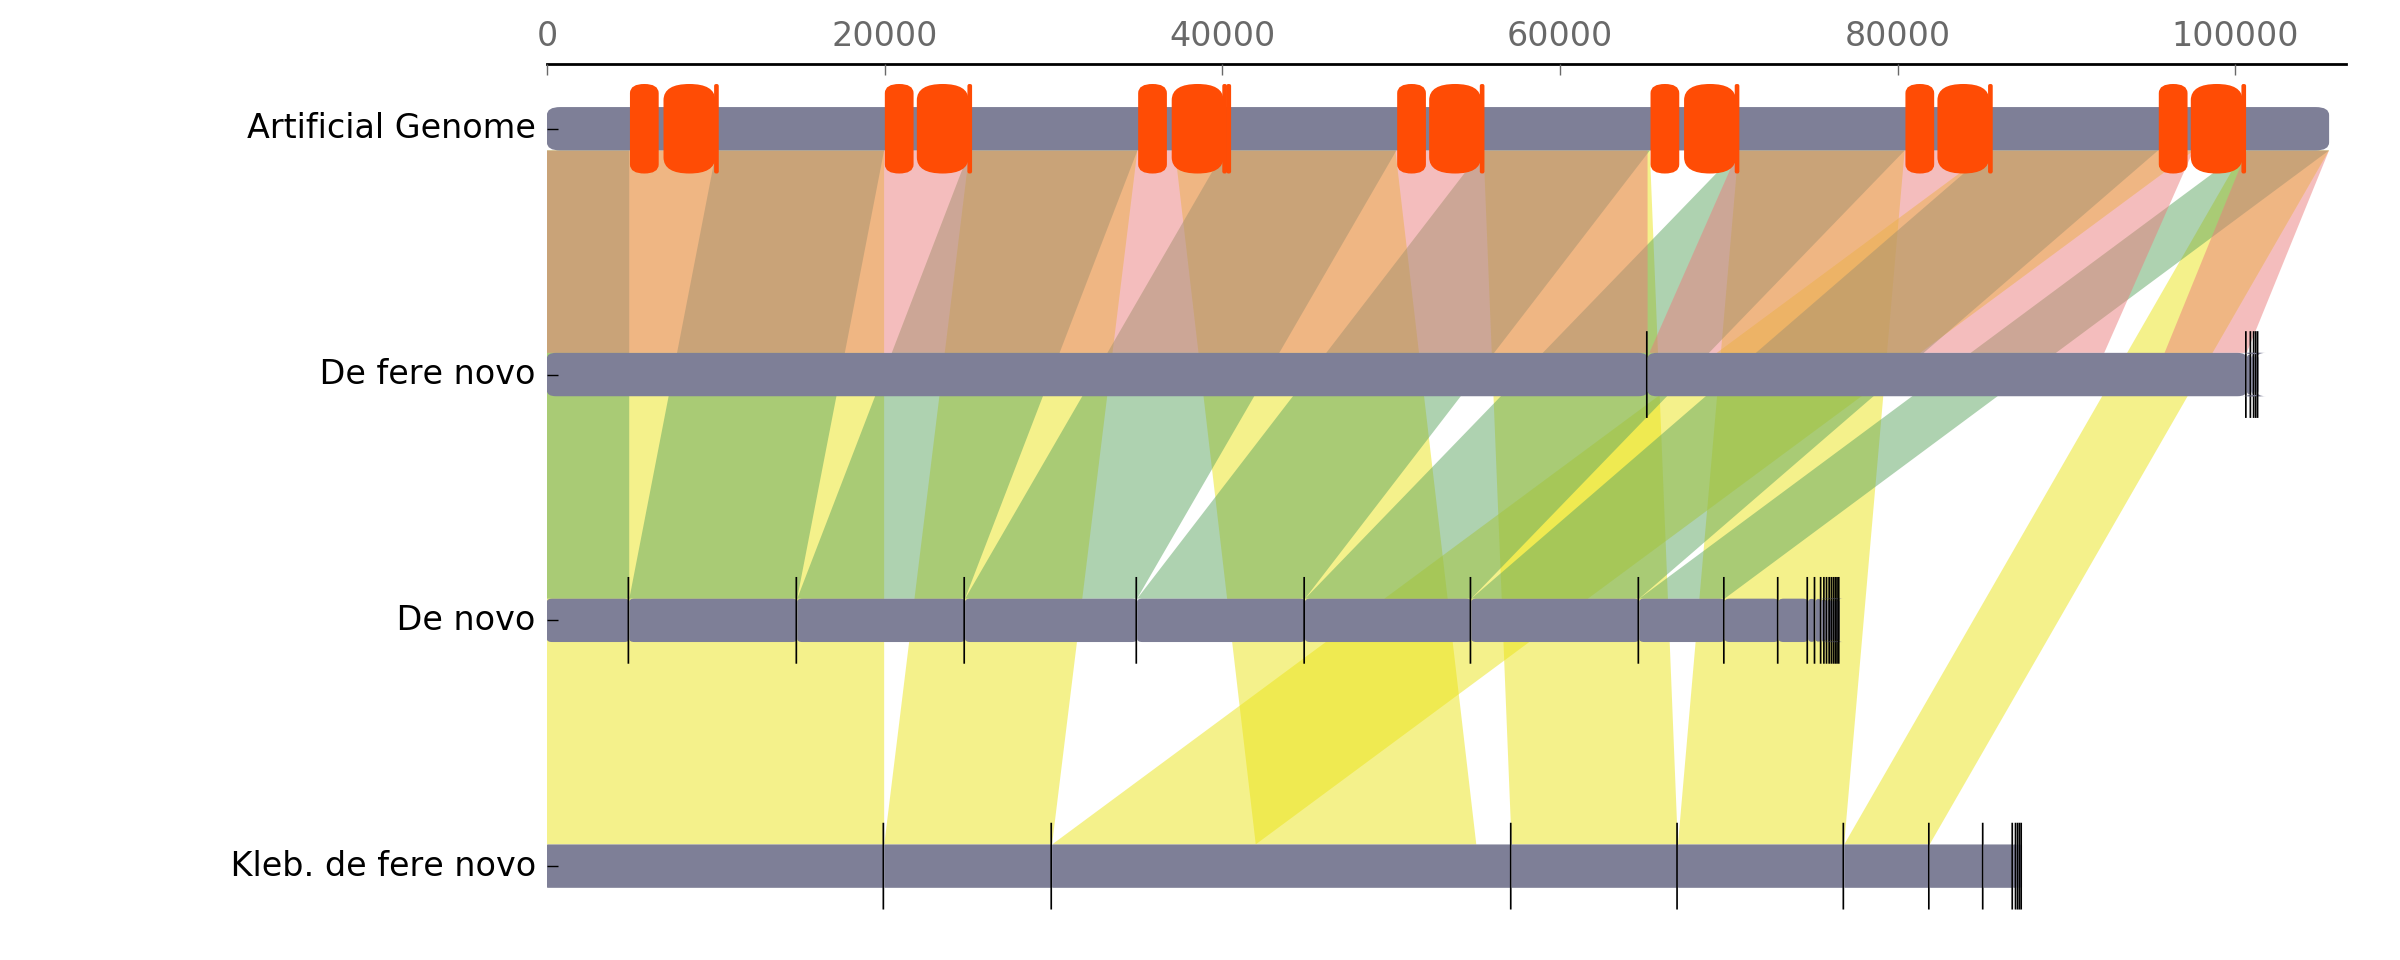
\includegraphics[width=1.2\columnwidth]{PrettyMauve}
    \caption{Representative Mauve output describing the results of riboSeed assemblies of simulated reads generated by pIRS from the concatenated \textit{E. coli} Sakai artificial chromosome. Red regions represent rRNA coding sequences, vertical black lines indicate boundaries between assembled contigs, and shading represents synteny. From top to bottom: artificial reference chromosome; rDNA clusters (red bars); \textit{de fere novo} assembly and \textit{de novo} assembly (both using \textit{E. coli } MG1655 as the reference). riboSeed's \textit{de fere novo} method assembles 4 of 7 rDNA regions, but the \textit{de novo} assembly recovers no rDNA regions correctly.
}
\label{fig:artificial}
\end{figure}
